% !TeX root = RJwrapper.tex
\title{GREENeR: An R Package to Estimate and Visualize Nutrients Pressures on Surface Waters}


\author{by Angel Udías, Bruna Grizzetti, Olga Vigiak, Alberto Aloe, Cesar Alfaro, and Javier Gomez}

\maketitle

\abstract{%
Nutrient pollution affects fresh and coastal waters around the globe. Planning mitigating actions requires tools to assess fluxes of nutrient emissions to waters and expected restoration impacts. Conceptual river basin models take advantage of data on nutrient emissions and concentrations at monitoring stations, providing a physical interpretation of monitored conditions, and enabling scenario analysis. The GREENeR package streamlines water quality model in a region of interest, considering nutrient pathways and the hydrological structure of the river network. The package merges data sources, analyzes local conditions, calibrate the model, and assesses yearly nutrient levels along the river network, determining contributions of load in freshwaters from diffuse and point sources. The package is enriched with functions to perform thorough parameter sensitivity analysis and for mapping nutrient sources and fluxes. The functionalities of the package are demonstrated using datasets from the Vistula river basin.
}

\hypertarget{introduction}{%
\section{Introduction}\label{introduction}}

Nitrogen and phosphorus are key nutrients that heavily impact aquatic ecosystems. Detecting primary sources of nutrient pollution and their downstream spread, alongside assessing achievable reductions through restoration policies, are crucial for effective natural resource management. They aid in identifying priority intervention areas and planning actions to restore the ecological balance of receiving waters.

Modelling tools can be useful to assess the impacts of future scenarios, policy measures, and climate changes at the regional and continental scale (Arheimer, Dahné, and Donnelly 2012; Bartosova et al. 2019; Beusen et al. 2022; Bouraoui et al. 2014; Ludwig et al. 2010; Seitzinger et al. 2005), and to check the coherence of different policy targets, for instance between water and agricultural policies. The assessment of policy scenarios requires a flexible and spatially detailed analysis to account for climatic, hydrological, and socio-economic gradients (Bruna Grizzetti et al. 2021).

Several types of models can be applied to predict the transport of nutrients in river basins Fu et al. (2019). Among them, statistical or conceptual models have the advantage of being readily applied in large watersheds. These model rely on calibration of few parameters for establishing links between emissions at sources and fate in the stream network. They take full advantage of nutrient emissions and concentrations data at monitoring stations, which are now accessible with increasing spatial and temporal resolution.

A classic example of river basin conceptual model is SPARROW (Smith, Schwarz, and Alexander 1997; Schwarz et al. 2006), which is widely applied in the U.S. to assess water quality over large regions. SPARROW has inspired the Geospatial Regression Equation for European Nutrient (GREEN) losses model (B. Grizzetti et al. 2005; Bruna Grizzetti, Bouraoui, and Aloe 2012; Bruna Grizzetti et al. 2021) which is adapted to European conditions. GREEN has been used for assessing the nutrient loads to the European seas (Bruna Grizzetti, Bouraoui, and Aloe 2012; Bruna Grizzetti et al. 2021), nitrogen retention in European freshwaters (Bruna Grizzetti, Bouraoui, and Aloe 2012; La Notte et al. 2017), and for policy scenario analysis (La Notte et al. 2017; Bouraoui et al. 2014; Leip et al. 2015; Malagó et al. 2019; Bruna Grizzetti et al. 2021). Despite their usefulness, this type of river basin models are seldom compiled as dedicated R packages, for example SPARROW has some scripts available to process information for and analysis of models results in the R environment.

The GREEN model application comprises several key steps, including data extraction and organization, data harmonization and integration, examination and validation of input data sets, model calibration and parameter selection, model run, and result visualization. All of these features are now integrated into an R package (\CRANpkg{GREENeR}) that comprises functions to streamline the process, evaluate and visualize all the steps, thus strengthening the robustness of model application.

\hypertarget{about-water-surface-nutrients-estimation-with-green}{%
\subsection{About water surface nutrients estimation with GREEN}\label{about-water-surface-nutrients-estimation-with-green}}

GREEN (B. Grizzetti et al. 2005; Bruna Grizzetti, Bouraoui, and Aloe 2012; B. Grizzetti, Bouraoui, and De Marsily 2008; Bruna Grizzetti et al. 2021) is a conceptual model to assess total nitrogen TN and total phosphorous TP from a region of interest (usually a river basin), accounting for both diffuse and point sources. The package allows the analysis of different scenarios of nutrient input in the region of interest, where ``scenario'' indicates a combination of annual time-series of inputs, such as nitrogen or phosphorus and the topological structure of the region. The model comprises several nutrient sources and pathways:

\begin{enumerate}
\def\labelenumi{\arabic{enumi}.}
\tightlist
\item
  agricultural diffuse sources include nutrients from mineral fertilisers and manure application, nitrogen crop and soil fixation. These sources undergo retention in the land phase (basin retention that account for e.g.~crop uptake and volatilization losses) before reaching the stream;
\item
  other diffuse emissions, such as from scattered dwellings (i.e., isolated houses and small agglomerations that are not connected to sewerage systems), and atmospheric nitrogen deposition (for nitrogen module) or background losses (for phosphorus module), are also reduced, e.g.~due to soil processes, before reaching the stream network;
\item
  point sources consist of urban and industrial wastewater discharges that are discharged into surface waters directly.
\end{enumerate}

\noindent Once in the river network, all nutrient loads are reduced by in-stream retention in rivers and lakes.

Basin retention of agriculture sources is a decay function proportional to the inverse of the total annual precipitation in the catchment. Conversely, river retention is a decay function proportional to the river length, considered as a proxy for water residence time. Finally, lake retention is simulated as a function of the lakes residence time and average depth.

The basin is divided into spatial subunits (called catchments), with a given area, a river reach, an inlet node, and an outlet node. The catchments are topologically connected from the headwaters to the outlet in a cascading sequence. The sequence of nutrient load accumulation through the stream network is defined by Shreve's order (Shreve 1966). Nutrient input from the different sources, basin and river retention are simulated in each catchment and routed through the river network. For each catchment \(i\) in the basin, the GREEN nutrient load \(L_i\) is estimated by the general equation:

\begin{equation}
  L_{i,y} = (1-Lret_i) \cdot (DSA_{i,y} \cdot (1-Bret_{i,y} )+ DSB_{i,y} + PS_{i,y} +U_{i,y} ) \cdot (1-Rret_i) 
\label{eq:green-nutrient-load}
\end{equation}

\noindent where \(L_{i,y}\) is the nutrient load at the catchment outlet-node (ton/yr) in \(y\) year; and the other variables represent different sources and sinks of nutrients.

Sources of nutrients are:

\begin{itemize}
\item
  \(DSA_{i,y}\). Annual nutrient diffuse sources on agricultural land in the catchment (ton/yr): mineral and manure fertilization, atmospheric nitrogen deposition, plant and soil fixation for TN; mineral and manure fertilization, and background losses for TP.
\item
  \(DSB_{i,y}\). Annual nutrient diffuse sources in the catchment related with scatter dwellings and atmospheric nitrogen deposition on non-agricultural land for TN (\(DSB_{i,y} = 0.38 \cdot FF_{i,y} \cdot AtmN_{i,y} + sd_{coeff} \cdot SdN_{i,y}\), where \(FF_{i,y}\) is the fraction of non-agricultural land cover in the catchment, and \(AtmN_{i,y}\) is the annual atmospheric nitrogen deposition on the catchment (ton/yr)); nutrient diffuse sources in the catchment related with scatter dwellings and background losses on non-agricultural areas for TP (\(DSB_{i,y} = sd_{coeff} \cdot SdP_{i,y})\).
\item
  \(PS_{i,y}\). Nutrient point sources in the catchment (ton/yr).
\item
  \(U_{i,y}\). Nutrient load from upstream catchments (ton/yr).
\end{itemize}

\noindent Sinks of nutrients are:

\begin{itemize}
\tightlist
\item
  \(Lret_i\) denotes the lake retention (fraction) of the \(i\) catchment. \(Lret\) is currently defined according to Kronvang et al. (2004), but limited to a \(10\%\) maximum reduction:
\end{itemize}

\begin{equation}
    Lret = \max\left(0.1, 1 - \frac{1}{1 + (dref / z) \cdot RT}  \right)
    \label{eq:lake-retention}
  \end{equation}

\noindent where \(z\) represents the average lake depth (m); \(RT\) is the hydraulic residence time (yr); and \(dref\) denotes a nutrient-related coefficient (\(dref = 7.3\) for TN and \(dref = 26\) for TP).

\begin{itemize}
\tightlist
\item
  \(Bret_{i,y}\) is the fraction of basin retention of the \(i\) catchment in \(y\) year:
\end{itemize}

\begin{equation}
    Bret_{i,y} = 1 - \exp(-alpha_P \cdot NrmInvRain_{i,y})
    \label{eq:basin-retention}
  \end{equation}

\noindent where \(NrmInvRain_{i,y}\) is the inverse of annual precipitation (mm) of the \(i\) catchment in \(y\) year, normalized by its maximum (Frank and Todeschini 1994). To keep basin retention coefficients comparable across regions, the minimum precipitation \(minPrec\) is set to \(50\) mm/y, and thus \(NrmInvRain_{i,y}\) is defined as

\begin{equation*}
    NrmInvRain_{i,y} = \frac{1 / \max(50,  precipitation_{i,y})}{(1 / minPrec)} 
  \end{equation*}

\begin{itemize}
\tightlist
\item
  \(Rret_i\) is the fraction of river retention of the \(i\) catchment:
\end{itemize}

\begin{equation}
    Rret_i = 1 - \exp(-alpha_L \cdot NrmLengthKm_i) 
    \label{eq:river-retention}
  \end{equation}

\noindent where \(NrmLengthKm_i\) is the length (km) of the catchment reach, normalized by the maximum in the dataset:

\begin{equation*}
    NrmLengthKm_i = \frac{\textrm{catchment length } i \textrm{ reach, in km}}{\max(\textrm{Reach length in the region, in km})}
  \end{equation*}

\noindent Since the maximum reach length depends on the region and its subdivision of network reaches, the calibrated coefficient \(alpha_L\) cannot be compared across regions that adopt different discretization. Note that basin retention varies from year to year according to annual precipitation, whereas the fraction of river and lake retention for a given catchment is constant in time.

Equation \eqref{eq:green-nutrient-load} is applied sequentially from the most upstream nodes to the basin outlet. The model parameters are:

\begin{enumerate}
\def\labelenumi{\arabic{enumi}.}
\tightlist
\item
  the basin retention coefficient (\(alpha_P\)), which together with annual precipitation regulates nutrient retention of diffuse agricultural sources (Equation \eqref{eq:basin-retention});
\item
  the river retention coefficient (\(alpha_L\): Equation \eqref{eq:river-retention}), which regulates the river retention per river km.
\item
  the fraction of domestic diffuse sources that reaches the stream network (\(sd_{coeff}\)).
\end{enumerate}

\hypertarget{about-the-package}{%
\section{\texorpdfstring{About the \pkg{GREENeR} package}{About the  package}}\label{about-the-package}}

\hypertarget{package-organization}{%
\subsection{Package organization}\label{package-organization}}

\noindent This work presents a new efficient and enhanced implementation of the model GREEN developed as an R package named \pkg{GREENeR}. \pkg{GREENeR} is developed in the R statistical software and provides tools and methods for applying GREEN to an area of interest and assessing annual time series of nutrient loads in a river network and at the basin outlet, plus contributions of nutrient sources to these loads. Some of the key features of the package comprise: a) functions for the creation of scenarios from data sources; b) computational efficiency; c) parallel-capable ; d) an extended suite of fine tuning options to control model calibration; e) built-in parameter sensitivity analysis; and f) functions to perform customised post-process analyses.

The functions of \pkg{GREENeR} package are arranged in three groups: i) functions to perform graphical summaries of model inputs; ii) functions to perform model parameters calibration and sensitivity analysis; iii) functions to compute, analyze and visualize through graphs and maps the model outputs, i.e.~total loads and contributions by source. The package supports parallel processing, which helps reduce the computational load in handling large basins.

The time-series can represent either historic (current or past) conditions that can be associated to observations for model calibration, or hypothetical conditions foreseen under theoretical changes (e.g.~to forecast results of nutrient management plans, or under climatic change).

A scenario contains:

\begin{enumerate}
\def\labelenumi{\arabic{enumi}.}
\item
  The geospatial geometry of the catchments of the region, which currently is defined according to the Catchment Characterisation and Modelling Database for European Rivers v2 (CCM2) (De Jager and Vogt 2007).
\item
  The annual time series (1990-2018) of nutrient inputs per catchment.
\item
  Additional catchment information (annual precipitation, annual forest fraction, lake retention, reach length).
\item
  Observed total load (TN or TP) from monitoring stations.
\end{enumerate}

\noindent Two historical scenarios, one for TN and one for TP, of the Lay basin (France) are provided with the \pkg{GREENeR} package. The Lay basin has an area of \(1971\) km\(^2\), and is divided into \(189\) CCM2 catchments. The mean catchment area is \(10.4\) km\(^2\). Nutrient observations comprised \(22\) TN entries from six monitoring stations and \(58\) TP data entries from eight monitoring stations (data from WISE Waterbase (EEA 2021)).

Further, in this article we present examples drawn for the TN historic scenario of the transboundary Vistula (Wisla) river basin, one of the largest river basins of Europe. The Vistula scenario comprises \(15465\) CCM2 catchments that compose the \(193.894\) km\(^2\) river basin, TN inputs for 1990-2018, as well as 1364 observed TN loads from 412 monitoring stations. The TN input dataset is part of the larger dataset created to assess nutrient concentration in the European freshwaters (Vigiak et al. 2023).

\hypertarget{key-functions-in-the-greener-package}{%
\subsection{Key functions in the GREENeR package}\label{key-functions-in-the-greener-package}}

A brief overview of the package and its main functions is given in Figure \ref{fig:schematic-diagram-GREENeR}.

\begin{figure}[H]
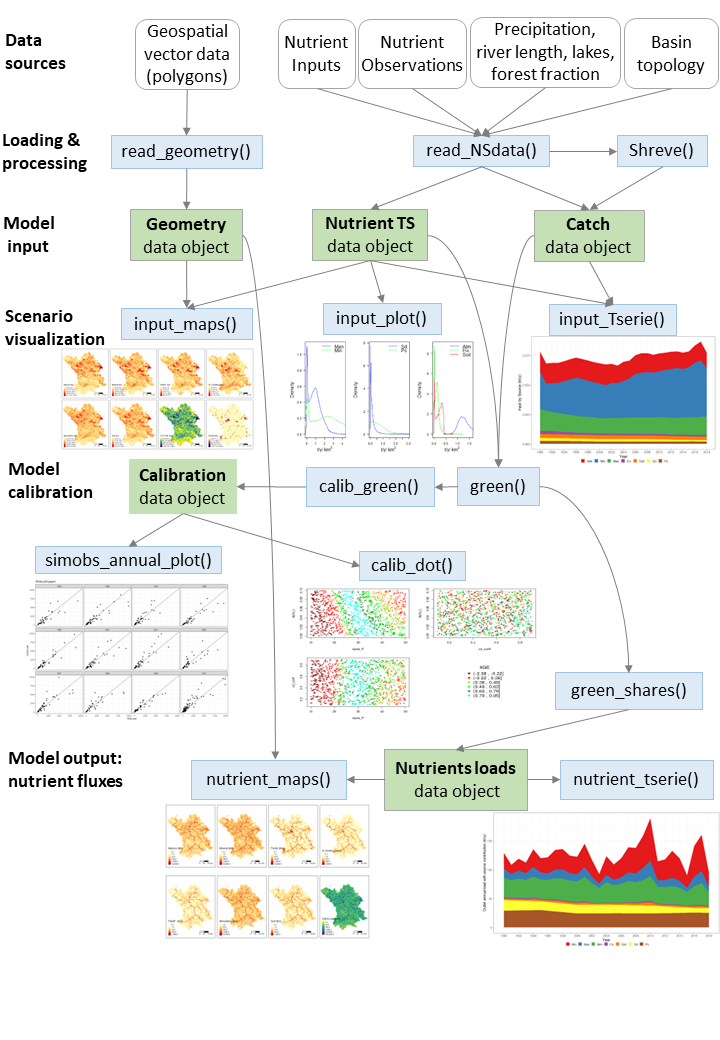
\includegraphics[width=0.9\linewidth,height=0.6\textheight]{figures/fig1} \caption{Schematic diagram of the procedure of GREENeR, including functions, data inputs and outputs, to estimate the nutrient loads. The green boxes represent data objects and the blue boxes represent the functions.}\label{fig:schematic-diagram-GREENeR}
\end{figure}

The key functions included in the package are:

\begin{itemize}
\item
  \texttt{read\_geometry()}: imports the geospatial vector format (shapefile or ESRI shapefile) with the spatial information of the catchments in R.
\item
  \texttt{read\_NSdata()}: imports the annual time series of nutrient inputs per catchment and type of nutrient source (manure, mineral fertilization, point sources, scatter dwellings), plus the forest fraction, and the observed annual nutrient loads from monitoring station data. The original data are stored in several comma-separated tables (CSV files).
\item
  \texttt{input\_maps()}: creates a map showing the mean nutrient load input by source.
\item
  \texttt{input\_plot()}: creates either a grouped barplot representing the average input load by source for the whole basin, or three density plots showing the distribution of nutrient sources.
\item
  \texttt{input\_Tserie()}: creates a time series plot showing basin inputs by source.
\item
  \texttt{shreve()}: returns the Shreve order of the catchments, a useful indicator of stream size, discharge, and drainage area (Strahler 1957) calculated based on the sum of the orders of up of upstream tributaries (Shreve 1966). Commercial GIS software usually provides a Shreve calculation function, but in other software, it is harder to find. In GREEN, the Shreve's order defines the cascade of upstream-downstream catchments.
\item
  \texttt{calib\_green()}: conducts sensitivity analysis of model calibration utilizing a Latin Hypercube Sampling (LHS) scheme (Manache and Melching 2004) for three model parameters. It evaluates model performance by calculating several ``goodness-of-fit'' (GoF) metrics (Refsgaard and Henriksen 2004) against available observations during the specified simulation period (years).
\item
  \texttt{select\_params()}: extracts the best parameter set according to a selected GoF metric from the object generated by the calibration function, \texttt{calib\_green()}.
\item
  \texttt{calib\_boxplot()}: creates a figure of boxplots that show the relationships between the best parameter sets determined by the specific GoF metric in each boxplot title, and six other commonly used hydrological metrics (Althoff and Rodrigues 2021; Mauricio Zambrano-Bigiarini 2014). In the lower panel, the figure also highlights the distribution of model parameters; the value of the best parameter set is marked as a red dot in each boxplot.
\item
  \texttt{region\_nut\_balance()}: runs the GREEN model with the selected parameter set, and returns the mean annual mass balance of nutrient fluxes for the whole simulation period of the region. The results of this function can be visualized using a Sankey diagram via the \texttt{N4\_sankey()} function.
\item
  \texttt{green()}: runs the GREEN model with the selected parameter set and returns nutrient load time series for the simulation period. It generates less information than the \texttt{green\_shares()} function, but its execution is faster, so it is used as a function for calibration iterations and is embedded in the \texttt{calib\_green()} function.
\item
  \texttt{green\_shares()}: runs the GREEN model with the selected parameter set and returns time series of nutrient loads and the contributions of each nutrient source in the simulation period. The results of the model can be examined by \texttt{nutrient\_tserie()} and \texttt{nutrient\_maps()} functions.
\item
  \texttt{scatter\_plot()}: generates dot plots correlating parameters realizations in the calibration data with GoF metric, visualizing the impact of each parameter on model outcomes. The plot vary based on selected GoF metric from \texttt{green\_calib()} function.
\item
  \texttt{simobs\_annual\_plot()}: generates scatter plots comparing model load predictions (PredictLoad) with observations (ObsLoad) for each year of the stimulation period.
\end{itemize}

\hypertarget{input-data-requirements}{%
\subsection{Input data requirements}\label{input-data-requirements}}

\pkg{GREENeR} requires information on the nutrient inputs, the topology, and the geospatial geometry of the region of interest. The spatio-temporal input data must include all nutrient source fields, and differs in the two nutrient scenarios (TN or TP). In the case of TN (e.g.~Figure \ref{fig:maps-TN}), fields are (Equation \eqref{eq:appendix1-1} in \protect\hyperlink{appendix-1}{Appendix 1}):

\begin{itemize}
\item
  \(Atmospheric\): Annual amount of atmospheric nitrogen deposition (ton/yr).
\item
  \(Mineral\): Annual amount of nitrogen from mineral fertilisers (ton/yr).
\item
  \(Manure\): Annual amount of nitrogen in manure fertilisers (ton/yr).
\item
  \(Fix\): Annual amount of nitrogen fixation by leguminous crops and fodder (ton/yr).
\item
  \(Soil\): Annual amount of nitrogen fixation in soils (ton/yr).
\item
  \(Sc. Dwellings\): Nitrogen input from scattered dwellings (ton/yr).
\item
  \(PointS\): Nitrogen input from point sources (ton/yr).
\end{itemize}

\begin{figure}[H]

\includegraphics[width=1\linewidth,height=0.35\textheight]{figures/fig2} \caption{Maps showing the mean annual TN inputs in the Vistula river basin in 1990-2018. The figure was generated with GREENeR input\_maps() function. TOT.Diff = sum of diffuse inputs.}\label{fig:maps-TN}
\end{figure}

\noindent In the case of TP, fields are (Equation \eqref{eq:appendix1-2} in \protect\hyperlink{appendix-1}{Appendix 1}):

\begin{itemize}
\item
  \(Background\): annual amount of phosphorus from background losses (ton/yr).
\item
  \(Mineral\): annual amount of phosphorus from mineral fertilisers (ton/yr).
\item
  \(Manure\): annual amount of phosphorus in manure fertilisers (ton/yr).
\item
  \(Sc. Dwellings\): phosphorus input from scattered dwellings (ton/yr).
\item
  \(PointS\): phosphorus input from point sources (ton/yr).
\end{itemize}

\noindent European datasets for 1990-2018 generated to assess historic and current nutrient fluxes (Vigiak et al. 2023) are available upon request. The model and the package are compatible with an external dataset and can be customized with local information as long as the data structure is respected.

In both nutrient cases, \pkg{GREENeR} needs additional annual catchment information:

\begin{itemize}
\item
  \(ForestFraction\): annual fraction (0-1) of non-agricultural land cover area in the catchment (\(FF\) in Equations \eqref{eq:appendix1-1} and \eqref{eq:appendix1-2}, in the \protect\hyperlink{appendix-1}{Appendix 1}).
\item
  \(Rain\): annual precipitation (mm, Equation \eqref{eq:basin-retention}).
\item
  \(LakeFrRet\): lake retention fraction (0-1) (\(Lret\) in Equation \eqref{eq:green-nutrient-load}, in the \protect\hyperlink{appendix-1}{Appendix 1}). Note, this differs for TN or TP scenarios (Equation \eqref{eq:lake-retention}). At European scale, average lake depth and hydraulic residence time can be obtained from HydroLAKES database (\url{https://www.hydrosheds.org/pages/hydrolakes}, Messager et al. (2016)).
\item
  Length: is the length (km) of the catchment reach (Equation \eqref{eq:river-retention}).
\end{itemize}

\noindent The catchment topology outlines the hydrological network configuration within the region. Each catchment must have a unique numerical identifier (HydroID)), to establish the network structure via a source HydroID and destination HydroID table. It is important to note that any outlet of the basin will be given as destination HydroID identifier ``-1''. Complementing the topology of the hydrologic network, the length of catchment reach should also be included (Equation \eqref{eq:river-retention}).

Finally, in order to calibrate the model, it is necessary to have some observed nutrient loads from monitoring stations associated to any catchment of the region. Ultimately, the quality, size, and spatial distribution of observed loads determine the robustness of the calibration process. In Europe, a large dataset of annual concentrations is publicly available (WISE Waterbase, EEA 2021), but annual flow must be derived from other sources (Bruna Grizzetti et al. 2021; Vigiak et al. 2023).

\hypertarget{performance-and-memory-use}{%
\subsection{Performance and memory use}\label{performance-and-memory-use}}

The \pkg{GREENeR} package performance and memory usage depends on the size of the region (number of catchments) and the number of years of the simulation. As a reference, the Danube basin (i.e.~the largest European basin, with \(138013\) catchments) TN dataset for 1990-2018 requires approximately \(389\) Mb of memory to store the annual data. Table \ref{tab:computational-requirements} shows the memory occupied by the scenarios for 6 European basins. In addition, it shows the computation times required in the execution of some key functions of the package. All executions were conducted on two computer configurations:

\begin{itemize}
\item
  CPU1: Desktop running window 10 with one Intel(R) Core i5-8259U CPU (4 cores, two threads per core) CPU at 2.30 GHz and 16 GB of RAM memory
\item
  CPU2: Workstation running Linux with one AMD EPYC 7352 (24 cores, two threads per core) CPU at 2.3 GHz and 128 GB of RAM memory
\end{itemize}

\noindent The time required for the execution of the different functions increases linearly with the number of catchments (or Shreve order) of the region (Table \ref{tab:computational-requirements}). The \texttt{calib\_green()} function is the most computationally demanding. However, the parallel implementation of this function drastically reduces the time required for this process. Calibration can be carried out in about 6 hours for practical implementation in large basins.

\begin{table}[htbp]\footnotesize
\caption{Computational requirements to run some \pkg{GREENeR} functions in six European basins scenarios of 29 years. The columns Shreve order, Area and Number of catchments characterize the size of each basin. Mem is the amount of memory occupied by the GREEN model scenario generated by \pkg{GREENeR} package. The \code{green()}, \code{green\_shares()} and \code{calib\_green()} columns show the computation time required to execute the corresponding \pkg{GREENeR} functions for each scenarios under CPU1 and CPU2 computer configurations. All runs of \code{calib\_green()} have been performed with 200 iterations. The reported times are the average of 5 runs of each process.}
\label{tab:computational-requirements}
\begin{tabular}{@{}lrrrrrrrrrr@{}}
\toprule
\begin{tabular}[c]{@{}l@{}}Basin\\ name\end{tabular} & \multicolumn{1}{l}{\begin{tabular}[c]{@{}l@{}}Shreve\\ order\end{tabular}} & \multicolumn{1}{l}{\begin{tabular}[c]{@{}l@{}}Area\\ ($\textrm{Km}^2$)\end{tabular}} & \multicolumn{1}{l}{\begin{tabular}[c]{@{}l@{}}Number of\\ catchments\end{tabular}} & \multicolumn{1}{l}{\begin{tabular}[c]{@{}l@{}}Mem\\ (MB)\end{tabular}} & \multicolumn{2}{c}{\begin{tabular}[c]{@{}c@{}}\code{green()}\\ (sec)\end{tabular}} & \multicolumn{2}{c}{\begin{tabular}[c]{@{}c@{}}\code{green\_shares()}\\ (sec)\end{tabular}} & \multicolumn{2}{c}{\begin{tabular}[c]{@{}c@{}}\code{calib\_green()}\\ (sec)\end{tabular}} \\ \midrule
                                                     & \multicolumn{1}{l}{}                                                       & \multicolumn{1}{l}{}                                                     & \multicolumn{1}{l}{}                                                               & \multicolumn{1}{l}{}                                                   & \multicolumn{1}{c}{CPU1}             & \multicolumn{1}{c}{CPU2}             & \multicolumn{1}{c}{CPU1}                 & \multicolumn{1}{c}{CPU2}                 & \multicolumn{1}{c}{CPU1}                 & \multicolumn{1}{c}{CPU2}                \\ \cmidrule(l){6-11} 
Lay                                                  & 95                                                                         & 1971                                                                     & 189                                                                                & 0.5                                                                    & 6                                    & 4                                    & 15                                       & 12                                       & 316                                      & 31                                      \\
Mi\~no                                                 & 2803                                                                       & 16985                                                                    & 5572                                                                               & 15.7                                                                   & 57                                   & 45                                   & 147                                      & 90                                       & 4110                                     & 394                                     \\
Seine                                                & 2902                                                                       & 75989                                                                    & 5793                                                                               & 16.3                                                                   & 77                                   & 55                                   & 177                                      & 106                                      & 6320                                     & 452                                     \\
Ebro                                                 & 9351                                                                       & 85611                                                                    & 18568                                                                              & 52.3                                                                   & 160                                  & 123                                  & 425                                      & 224                                      & 10876                                    & 995                                     \\
Vistula                                              & 7757                                                                       & 193894                                                                   & 15465                                                                              & 43.6                                                                   & 132                                  & 100                                  & 314                                      & 187                                      & 9004                                     & 814                                     \\
Danube                                               & 69505                                                                      & 802032                                                                   & 138013                                                                             & 388.6                                                                  & 1120                                 & 766                                  & 2855                                     & 1108                                     & 94682                                    & 5638                                    \\ \bottomrule
\end{tabular}
\end{table}

\hypertarget{estimating-nutrient-loads-using-the-package}{%
\section{\texorpdfstring{Estimating nutrient loads using the \pkg{GREENeR} package}{Estimating nutrient loads using the  package}}\label{estimating-nutrient-loads-using-the-package}}

The entire procedure is summarized on Figure \ref{fig:schematic-diagram-GREENeR}. Once the input data have been uploaded, the region scenario (Nutrient data and Catch data) is generated. The \texttt{calib\_green()} function explores the parameter set ranges with LHC scheme, calculating GoF of parameter sets. Sensitivity analysis of its results is conducted to determine the best parameter set. Finally, the \texttt{green\_shares()} function is used to estimate the nutrient loads and source apportionment (i.e.~contribution to loads by source), per year and per catchment.

\hypertarget{scenario-preparation}{%
\subsection{Scenario preparation}\label{scenario-preparation}}

Assembling input data for running the GREEN model is time consuming. To facilitate the process, the \texttt{read\_NSdata()} function assembles and organises annual information to generate a list of two objects: \texttt{Nutrient\ Time\ Series\ Data\ Object} and \texttt{Catch\ Data\ Object} of GREEN scenario. It needs four CSV files with specific data, namely:

\begin{itemize}
\item
  Time-series of annual nutrient inputs per catchment.
\item
  Time-series of annual observed loads at monitoring stations.
\item
  Basin topology and lake properties.
\item
  Other: precipitation, forest fraction, reach length.
\end{itemize}

\noindent The spatial identifiers (HydroID) and temporal (year) units must be coherent in all the files. Besides organizing the input data, the \texttt{read\_NSdata()} function also calculates the Shreve order of each catchment, normalises the precipitation (calculating \(NrmInvRain_{i,y}\)) and the reach length (\(NrmLengthKm_i\)).

\begin{verbatim}
csv_path <- "data/csv/"
scen <- read_NSdata(csv_path,"nutrients.csv","monitoring.csv", "forestFr.csv",
                    "precipitation.csv","topology.csv", "lakeProperties.csv",
                    "length.csv")
nutrient <- scen[[1]]
catch    <- scen[[2]]
\end{verbatim}

\noindent The \texttt{shreve()} function can calculate the Shreve order independently based on the topology of the basin:

\begin{verbatim}
shreve_order <- shreve(catch) 
\end{verbatim}

\noindent Finally, the geospatial geometry of the catchments should be uploaded to enable the visualisation functionalities in map form. The \texttt{read\_geometry()} function loads the geometry information file, i.e.~a geospatial vector with the geometry of the catchment region:

\begin{verbatim}
geometry <- read_geometry(file = "data/shapes/Wisla.shp")
\end{verbatim}

\noindent The geo-reference information, geometry and attributes of the spatial entities must be in a shapefile format (.shp), editable with ArcGIS or similar software. The identifiers of each catchment (HydroID) must be consistent with those in the CSV files of the scenario dataset.

Once the scenario has been generated, the library includes functions to examine the nutrient sources in a basin, and explore their distribution over time or in space. The \texttt{input\_plot()} function provides annual average nutrient loads for the whole period and density plots of nutrient loads. The \texttt{input\_Tserie()} function allows to examine the temporal evolution of the inputs, whereas the \texttt{input\_maps()} function generates maps of nutrient inputs distribution in the basin (Figure \ref{fig:maps-TN}).

\begin{verbatim}
input_maps(nutient, catch, geometry, "Wisla", "gr1")
\end{verbatim}

\hypertarget{calibration-procedure-and-sensitivity-analysis}{%
\subsection{Calibration procedure and sensitivity analysis}\label{calibration-procedure-and-sensitivity-analysis}}

The calibration process is essential to find a suitable set of parameters for the model. In \pkg{GREENeR} package, the core function \texttt{calib\_green()} enables to run a parameter sensitivity analysis and concurrently assessing the model performance according to several GoF metrics.

Sensitivity Analysis (SA) investigates how the variation in the output of a numerical model can be attributed to variations of its input factors. SA aims at identifying the most influential inputs or parameters, and quantifying how much they contribute to the variability/uncertainty of the model outputs. SA provides information on how much of the output variance is controlled by each parameter, or combination of parameters. SA is increasingly being used in environmental modelling for a variety of purposes, including uncertainty assessment, model calibration and diagnostic evaluation, dominant control analysis, and robust decision-making (Pianosi et al. 2016; Saltelli, Annoni, et al. 2011; Butler et al. 2014; Norton 2015; Mannina et al. 2018). This is achieved by running the model for many samples of the parameter space to determine their impact on the model outputs. SA allows identification of the parameters and input variables that strongly influence the model response (model output). Conversely, it may be of interest to the modeller to verify that although some model parameters may not be very well established they do not significantly contribute to output uncertainty. Saltelli, Tarantola, and Campolongo (2000) single out three main classes of SA methods: screening, local, and global methods. Local sensitivity analysis methods focus on assessing the impact of small variations in the input values of a model on the output results. Global sensitivity methods seek to understand how variations in the full range of input values affect the results. Puy et al. (2022) provide a comprehensive overview of several R packages for performing global sensitivity analysis.

Screening methods are economical and qualitative methods. Only screening methods are included in this implementation of the library as they provide a quick assessment of the relative importance of variables. This is particularly useful in exploratory studies and in cases where an initial subset of relevant variables needs to be identified.

Adequate sampling of parameter space is very important in model calibration. Several studies of uncertainty analysis in water resources problems (Melching and Bauwens 2001) concluded that Monte Carlo simulation and Latin Hypercube Sampling (LHS) (McKay, Beckman, and Conover 1979; Carnell 2012) methods are very powerful, robust, and flexible. Other approaches are possible (Mauricio Zambrano-Bigiarini 2014), but the LHS has the advantage that it is easily parallelisable, it explores the full range of parameter sets, it does not direct the search depending on the values of previous iterations like other optimisation methods (gradients, genetic algorithms, etc.), and is therefore independent of the GoF metric. This allows performing a posteriori sensitivity analysis for several metrics without having to repeat the process.

The \texttt{calib\_green()} function computes 15 GoF metrics (Althoff and Rodrigues 2021; Mauricio Zambrano-Bigiarini 2014) (listed in \protect\hyperlink{appendix-2}{Appendix 2}), and returns an object with all parameter sets generated by the LHS and the corresponding GoF scores. Running \texttt{calib\_green()} requires the following settings:

\begin{enumerate}
\def\labelenumi{\arabic{enumi}.}
\item
  The expected ranges for each parameter. The ranges are defined by two vectors of three values, one for the lower limits and one for the upper limits of the three parameters. The values correspond to each model parameter in sequence: \(alpha_P\) (Equation \eqref{eq:basin-retention}), \(alpha_L\) (Equation \eqref{eq:river-retention}), and \(sd_{coeff}\) (Equations \eqref{eq:appendix1-1} and \eqref{eq:appendix1-2}).
\item
  The number of iterations to be performed during the calibration process. The higher the number of iterations, the more likely it is to achieve good results, but the longer the computation time. Depending on the basin and parameter range width, it is recommended to run at least 200 iterations to have enough information to continue the calibration process.
\item
  The years to be included in the calibration process.
\end{enumerate}

\begin{verbatim}
n_iter <- 2000  
low <- c(10, 0.000, 0.1)   
upp <- c(50, 0.1, 0.9)    
years <- c(1990:2018)

calibration <- calib_green(nutrient, catch, n_iter, low, upp, years)
\end{verbatim}

\noindent The calibration process is automatically parallelised by the package and uses all computer cores except one. The computation time depends on the computer, the number of catchments in the basin, and the number of iterations (Table \ref{tab:computational-requirements}). The \texttt{calib\_green()} function returns a data frame with a row for each iteration with parameter values and the resulting 15 GoF metric scores. An example of four parameter sets is shown below (cut to the first five GoF metrics).

\begin{verbatim}
#>     alpha_P    alpha_L  sd_coeff    NSE   mNSE   rNSE    KGE PBIAS %
#> s1 39.31203 0.07628558 0.6325056 0.5623 0.6452 0.9595 0.2512   -44.1
#> s2 35.06049 0.05510985 0.1577470 0.6733 0.6948 0.9563 0.3763   -36.3
#> s3 28.34947 0.04418381 0.7209566 0.8690 0.7737 0.8998 0.7926    -1.7
#> s4 40.73533 0.01351723 0.6195734 0.8370 0.7734 0.9607 0.6292   -22.6
\end{verbatim}

\noindent The selection of the appropriate GoF metric(s) for calibration and evaluation of hydrological models can be challenging even for very experienced hydrologists. Choosing the right GoF metric for model calibration largely depends on the overall study scope, which defines the main interest (e.g.~high or low load, upper or lower catchment area), and on the available observation dataset (size and quality) (Kumarasamy and Belmont 2018). Automated calibration typically relies, often exclusively, on a single GoF metric, with the Nash-Suttclife efficiency (NSE) been the most frequently used metric in hydrological models (Hoshin V. Gupta et al. 2009; Westerberg et al. 2011; Wöhling, Samaniego, and Kumar 2013). As described in Singh and Frevert (2002), a single criterion is inherently predisposed to bias towards certain components of the data time series. Automated procedures may be improved by using more than one criteria as discussed by Hoshin Vijai Gupta, Sorooshian, and Yapo (1998). Although automation can help the calibration process become more objective, efficient and practical, it is not a substitute for expert hydrologic intuition and understanding. Whether automated or manual calibration is used, a common approach is to adjust the parameters that display the highest sensitivity (Madsen 2003; Doherty and Skahill 2006).

\pkg{GREENeR} includes several functions to assist in selecting the best parameter set. The \texttt{calib\_boxplot()} function shows (Figure \ref{fig:boxplot-vistula-river}) relationships between best parameter sets chosen according to one GoF parameter (title of each boxplot) in relation to six most frequently used metrics. Additionally, in the lower panel, the figure shows the distribution of model parameters in the most performing subset of parameter sets. The best parameter set according to each GoF metrics is marked as a red dot in each boxplot (Figure \ref{fig:boxplot-vistula-river}).

\begin{verbatim}
calib_boxplot(calibration, rate_bs = 5)
\end{verbatim}

\begin{figure}[H]
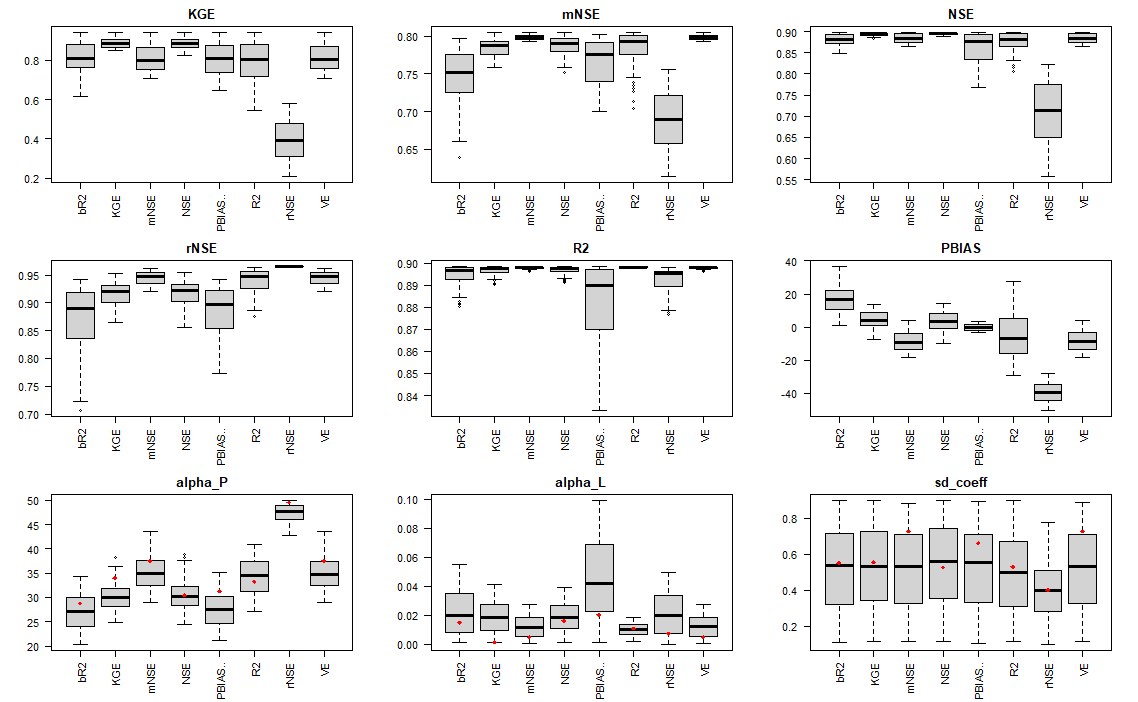
\includegraphics[width=1\linewidth,height=0.4\textheight]{figures/fig3} \caption{Calibration results for the Vistula river basin (TN Scenario). The figure displays the output of the calib\_boxplot() function, and compare several GoF metrics (bR2, KGE, mNSE, NSE, PBIAS, R2, rNSE, VE) with each other and with the model parameters distributions. The top two rows show boxplots of each metric (specified in the title) with others (in the x labels). The lowest row shows the parameter value distributions for the top 5\% (or another threshold indicated in rate\_bs parameter of the function) parameter sets ranked according to the GoF metrics in the x label. The red dots represent the best parameter values for each boxplot.}\label{fig:boxplot-vistula-river}
\end{figure}

\noindent The \texttt{select\_params()} function extracts the parameter set that scored the best GoF metric of choice from the calibration result object.

\begin{verbatim}
best_params <- select_params(calibration, param = "NSE")

alpha_P  <- best_params$alpha_P
alpha_L  <- best_params$alpha_L 
sd_coeff <- best_params$sd_coeff
\end{verbatim}

\noindent It is not recommended to use the parameters extracted by the \texttt{select\_params()} function without having performed an analysis of all the calibration results. Instead, alternative parameter sets (according to different GoF) should be compared before making the final selection.

Screening and SA of model parameters can be done via the \texttt{scatter\_plot()} and \texttt{calib\_dot()} functions of \pkg{GREENeR} package. The \texttt{scatter\_plot()} function shows all parameter realizations in the LHS dataset against a selected GoF metric to visualize the influence of each parameter on the metric scores. The result depends on the GoF metric of choice (any metric calculated with \texttt{calib\_green()} can be selected) (Figure \ref{fig:scatter-plot-vistula-river}).

\begin{verbatim}
scatter_plot(calibration, param = "R2")
\end{verbatim}

\begin{figure}[H]
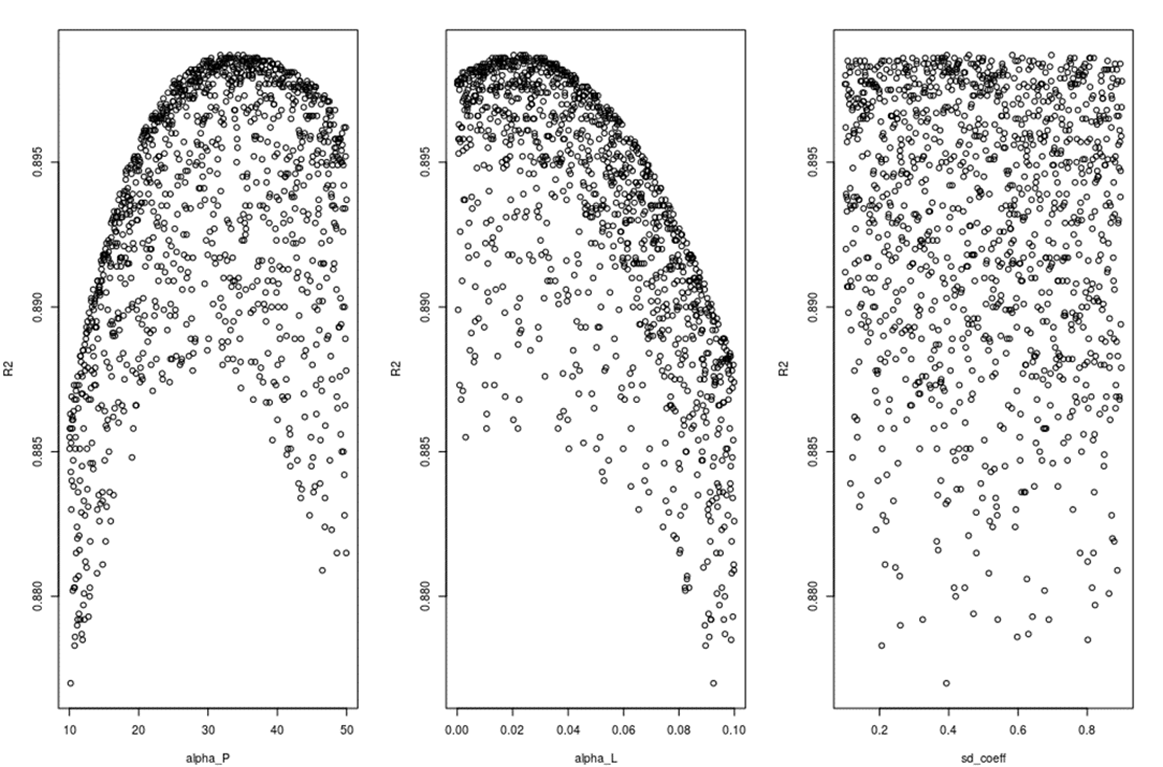
\includegraphics[width=1\linewidth,height=0.31\textheight]{figures/fig4} \caption{Scatter plots of model parameters against R2 metric generated by the scatter\_plot() function for the Vistula river basin (TN).}\label{fig:scatter-plot-vistula-river}
\end{figure}

\noindent Figure \ref{fig:scatter-plot-vistula-river} example shows that the highest R2 are achieved for values of the parameter \(alpha_P\) around \(33.3\) and for the parameter \(alpha_L\) around \(0.025\), whereas the model is insensitive to the \(sd_{coef}\) parameter. Further, \texttt{scatter\_plot()} function helps check if the parameter ranges defined in the search were suitable, or if the number of iterations was sufficient. In Figure \ref{fig:scatter-plot-vistula-river}, the best values of the parameters \(alpha_P\) and \(alpha_L\) are in the central part of the plots, thus the search parameter ranges were appropriate, and the distribution of dots is sufficient to visualize the effect of each parameter, indicating that the number of iterations was adequate.

The \texttt{calib\_dot()} function shows the distribution of parameters in relation to each other for a chosen GoF metric, and highlights potential correlations between parameters (Figure \ref{fig:dot-plot-vistula-river}).

\begin{verbatim}
calib_dot(calibration, param = "KGE") 
\end{verbatim}

\begin{figure}[H]
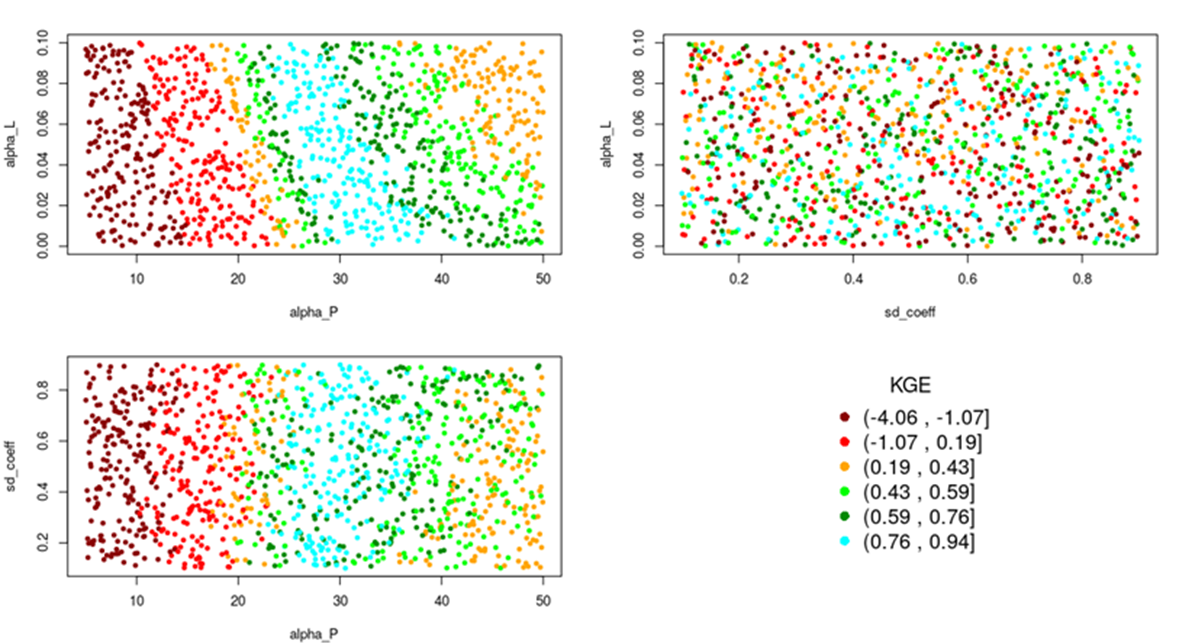
\includegraphics[width=1\linewidth,height=0.35\textheight]{figures/fig5} \caption{Dot plots of parameter pairs for the Kling-Gupta efficiency (KGE) generated by the calib\_dot() function for the Vistula river basin (TN).}\label{fig:dot-plot-vistula-river}
\end{figure}

\noindent In Figure \ref{fig:dot-plot-vistula-river}, the Kling-Gupta Efficiency metric (KGE, Althoff and Rodrigues 2021) shows interactions between \(alpha_P\) and \(alpha_L\), i.e.~a higher \(alpha_P\) should be associated to a lower \(alpha_L\) for achieving similar KGE. The best \(alpha_P\) values identified for both R2 and KGE metrics are similar, whereas \(alpha_L\) values vary considerably (see also Figure \ref{fig:boxplot-vistula-river}).

The \pkg{GREENeR} package includes two useful model calibration functions: \texttt{compare\_calib()} and \texttt{simobs\_annual\_plot()}. \texttt{compare\_calib()} shows a scatter plot that compares observed data points with corresponding values predicted by two parameter sets. Figure \ref{fig:compare-calib-vistula-river} displays a plot generated by the \texttt{compare\_calib()} for the Vistula (TN) basin scenario when using the best parameter sets based on NSE and rNSE metrics. The plot reveals that when rNSE parameter set result in an underestimation of loads in the upper range.

\begin{verbatim}
metrics <- c("NSE","rNSE")
compare_calib(nutrient, catch, alpha_p1 = 31, alpha_l1 = 0.02, sd_coef1 = 0.6,
              alpha_p2 = 50, alpha_l2 = 0.01, sd_coef2 = 0.6, years = c(1990:2018), 
              name_basin = "Wisla", metrics)
\end{verbatim}

\begin{figure}[H]
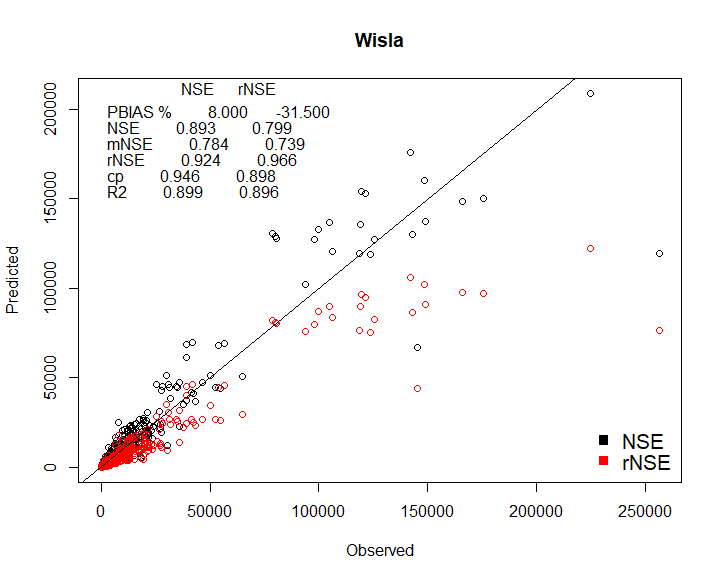
\includegraphics[width=1\linewidth,height=0.45\textheight]{figures/fig6} \caption{Result of compare\_calib() for the Vistula river basin (TN), comparing the best set of parameters selected according to the NSE and rNSE metrics.}\label{fig:compare-calib-vistula-river}
\end{figure}

\noindent The \texttt{simobs\_annual\_plot()} function compares observed and predicted values over the years (Figure \ref{fig:simobs-annual-plot-vistula-river}), which identifies erroneous model performance or data distribucion problems over time.

\begin{verbatim}
year_range <-  c(1994, 1996:2001, 2006:2009, 2012)      
simobs_annual_plot(nutrient, catch, alpha_P, alpha_L, sd_coeff, year_range, 
                   name_basin = "Wisla", max_value = 10000)
\end{verbatim}

\begin{figure}[H]
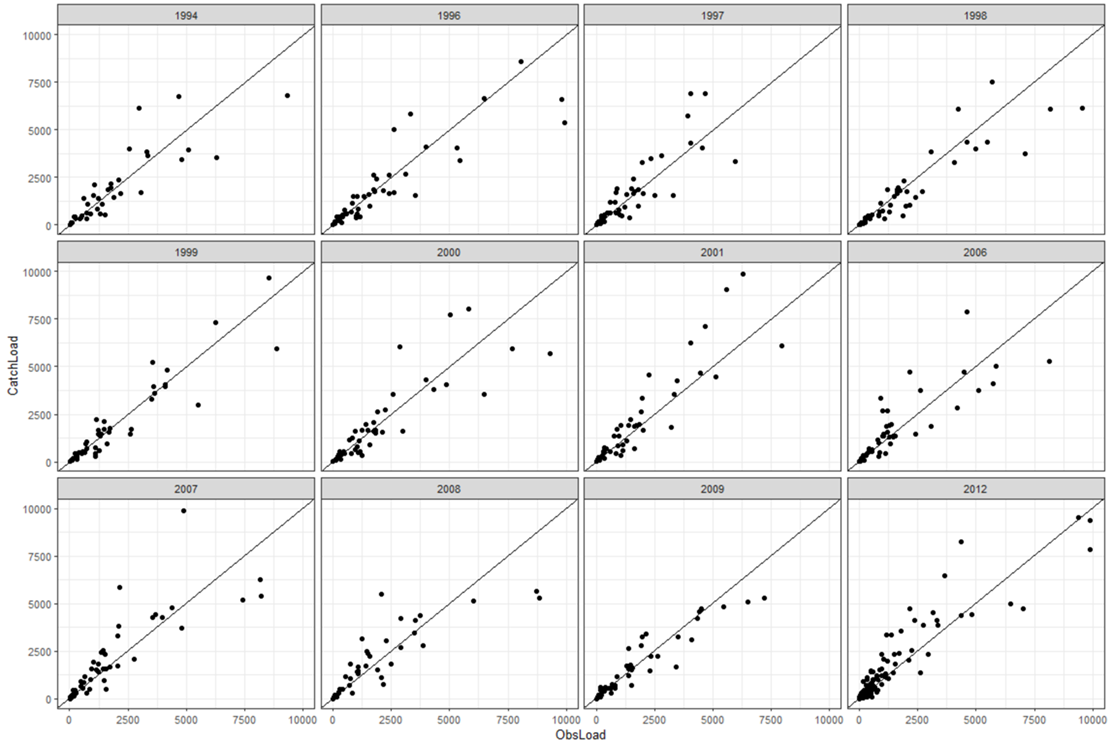
\includegraphics[width=1\linewidth,height=0.3\textheight]{figures/fig7} \caption{Result of the simobs\_annual\_plot() for the Vistula river basin (TN), with the parameter set selected for highest NSE and limiting the plots to the interval between 0 and 10000}\label{fig:simobs-annual-plot-vistula-river}
\end{figure}

\hypertarget{estimation-of-catchment-nutrient-loads-and-contribution-in-the-basin}{%
\subsection{Estimation of catchment nutrient loads and contribution in the basin}\label{estimation-of-catchment-nutrient-loads-and-contribution-in-the-basin}}

Once the most appropriate parameter set has been selected, it is possible to run the model to estimate nutrient loads in the region. The \texttt{green\_shares()} function runs GREEN with the selected parameter set and returns catchment nutrient loads and the contributions by source in the simulation period.

The \texttt{nutrient\_tserie()} function shows the temporal evolution of the total load at the basin outlet in the simulation period with contributions by sources (Figure \ref{fig:total-TN-vistula-river}). Other options of the function show nutrient loads in different zones of the basin (upper, central and lower part).

\begin{verbatim}
nutrient_load <- green_shares(nutrient, catch, alpha_P, alpha_L, sd_coeff, years)
nutrient_tserie(nutrient_load, geometry, "Wisla basin", "gr3")
\end{verbatim}

\begin{figure}[H]
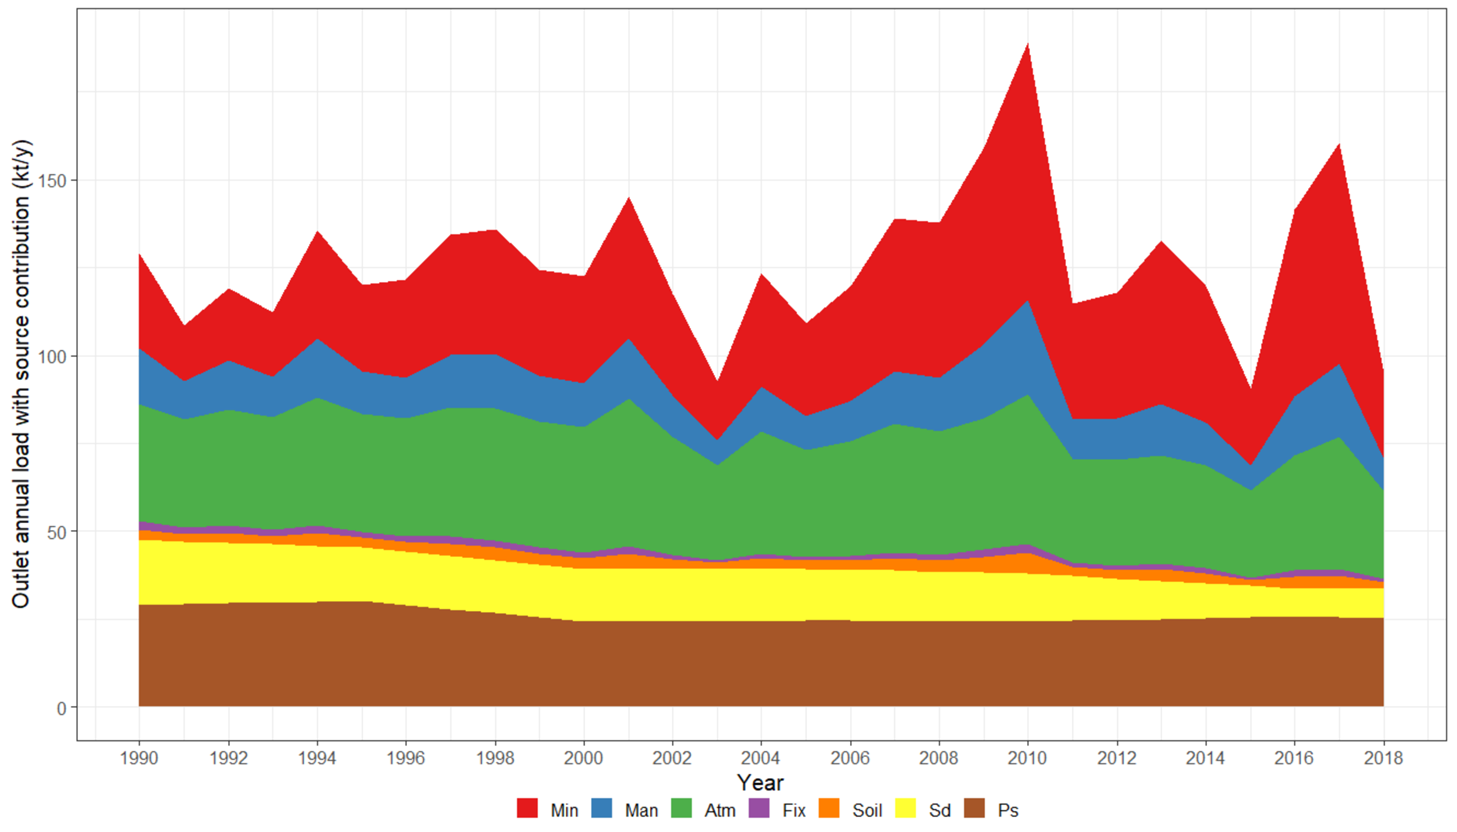
\includegraphics[width=0.9\linewidth,height=0.25\textheight]{figures/fig8} \caption{TN load at the Vistula river basin outlet from 1990 to 2018. Colors indicate the contribution of different sources (Min = mineral, Man = manure, Atm = atmospheric deposition, Fix = crop fixation, Soil = soil fixation, Sd = scattered dwellings and Ps = point sources).}\label{fig:total-TN-vistula-river}
\end{figure}

\noindent The \texttt{nutrient\_maps()} function uses the object returned by \texttt{green\_shares()} to generate maps of the distribution of nutrient loads by source for a given year or as the mean for several years (Figure \ref{fig:maps-TN-vistula-river}). The results are shown in logarithmic scale to improve the visualization as nutrient loads in a region may vary over several orders of magnitude. Alternative options of the function show the total load at the outlets of the catchment or the specific loads (i.e.~load per catchment area; in kt/km\(^2\)/y).

\begin{verbatim}
map_title <- "Output Loads for the Vistula basin"
nutrient_maps(nutrient_load, geometry, map_title, "gr1", legend_position = 1)
\end{verbatim}

\begin{figure}[H]
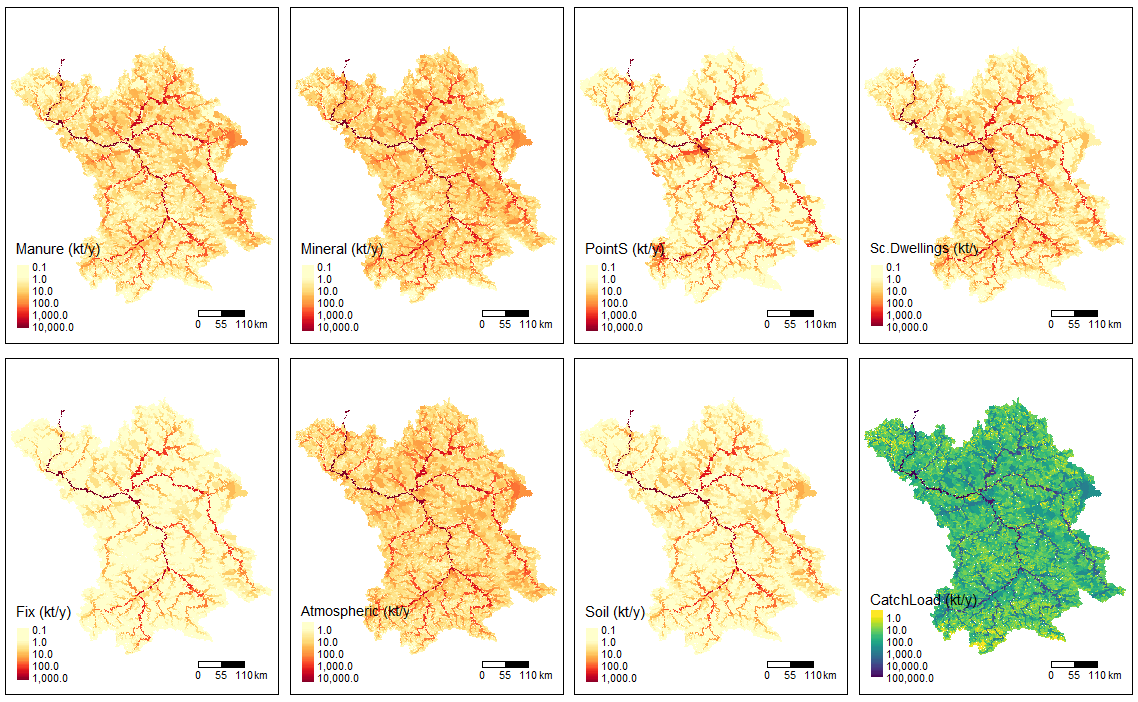
\includegraphics[width=1\linewidth,height=0.25\textheight]{figures/fig9} \caption{Maps of TN loads in the Vistula river basin by different sources and in total (the sum of all other maps, bottom right), in logarithm scale as generated with nutrient\_maps() function.}\label{fig:maps-TN-vistula-river}
\end{figure}

\hypertarget{estimation-of-nutrient-fluxes-and-sources-contribution-in-the-basin}{%
\subsection{Estimation of nutrient fluxes and sources contribution in the basin}\label{estimation-of-nutrient-fluxes-and-sources-contribution-in-the-basin}}

The \texttt{region\_nut\_balance()} function runs GREEN with the selected parameter set, and returns the nutrient mass balance and fluxes of the region (mean value for the simulation period). The results of this function can be visualized in a Sankey diagram with the function \texttt{N4\_sankey()} (Figure \ref{fig:sankey-vistula-river}) .

\begin{verbatim}
nut_bal <- region_nut_balance(nutrient, catch, alpha_P, alpha_L, sd_coeff, 
                              years)
sank <- N4_sankey(nut_bal)
\end{verbatim}

\begin{figure}[H]
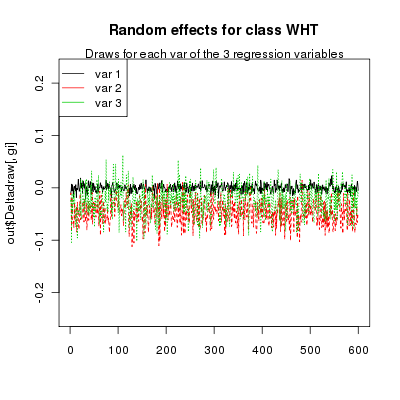
\includegraphics[width=1\linewidth,height=0.35\textheight]{figures/fig10} \caption{Sankey plot for the Vistula river basin for TN scenario, average for period 1990-2018. The plot represents nitrogen input sources on the left (Min=mineral, Man=manure, Atm=atmospheric deposition, Fix=crop fixation, Soil=soil fixation, Sd=scattered dwellings and Ps=point sources), and nitrogen sinks (land, river and lake retention) and outlet discharge (load to outlet) on the right. The bars in the middle visualize nitrogen agricultural diffuse sources and loads to the stream network.}\label{fig:sankey-vistula-river}
\end{figure}

\hypertarget{conclusion}{%
\section{Conclusion}\label{conclusion}}

The \pkg{GREENeR} package provides several functions to assess nutrient pressures in fresh and coastal waters based on the GREEN model (Bruna Grizzetti, Bouraoui, and Aloe 2012; Bruna Grizzetti et al. 2021). It allows assessing annual nutrient loads and concentrations throughout the river network and at river outlets, as well as the contributions of diffuse and point sources to the total load. \pkg{GREENeR} includes functions to route nutrient sources in a region, considering different pathways and the hydrological structure of the river network. The package is enriched by functions that aid selecting the set of parameters that best suits the study scope. Several functions assist in the preparation of scenarios by assembling input data from the appropriate sources, and in visualising inputs and nutrient fluxes in space and time. The version of the GREEN model implemented in the package is computationally efficient and includes parallel running capabilities for the calibration process, greatly reducing the time required for large basins or regional applications, e.g.~at continental scale as in (Vigiak et al. 2023).

\hypertarget{acknowledgements}{%
\section{Acknowledgements}\label{acknowledgements}}

This work has been partially supported by grant XMIDAS, ref. PID2021-122640OB-I00, funded by the Spanish Ministry of Science and Innovation.

\hypertarget{appendix}{%
\section{Appendix}\label{appendix}}

\hypertarget{appendix-1}{%
\subsection{Appendix 1}\label{appendix-1}}

Diffuse and point sources are defined differently for each nutrient module, i.e.~nitrogen or phosphorus. Equation \eqref{eq:appendix1-1} formulates the general GREEN function stated in equation \eqref{eq:green-nutrient-load} in the case of nitrogen. In GREEN nitrogen model, the total nitrogen load \(L_i\) of catchment \(i\) is estimated as:

\begin{equation}
\begin{split}
   L_i = (1 - Lret_i) \cdot ((MinN_i + ManN_i + FixN_i + SoilN_i + (1 - FF_i) \cdot AtmN_i) \cdot \\ (1 - Bret_i) + 0.38 \cdot FF_i \cdot AtmN_i + sd_{coeff} \cdot SdN_i + PsN_i + U_i) \cdot (1 - Rret_i)  
\end{split}
\label{eq:appendix1-1}
\end{equation}

\noindent where \(MinN_i\) is the annual amount of nitrogen from mineral fertilisers (ton/yr); \(ManN_i\) is the annual amount of nitrogen in manure fertilisers (ton/yr); \(FixN_i\) is the annual amount of nitrogen fixation by leguminous crops and fodder (ton/yr); \(SoilN_i\) is the annual amount of nitrogen fixation by bacteria in soils (ton/yr); \(AtmN_i\) is the annual nitrogen deposition from atmosphere (ton/yr); \(FF_i\) is the non-agricultural land cover in the catchment (fraction); \(SdN_i\) is the nitrogen input from scattered dwellings (ton/yr); \(PsN_i\) is the nitrogen input from point sources (ton/yr); and, finally, \(U_i\) is the nitrogen load from upstream catchments (ton/yr).

Note that nitrogen atmospheric deposition losses are split into two parts, i.e.~inputs to agricultural land, which undergo the basin retention (such as crop uptake) that depends on annual precipitation, while in forest areas they are reduced by a fixed rate, before entering into the stream. The contribution of atmospheric nitrogen deposition in non-agricultural land is thus estimated as \(0.38 \cdot FF \cdot AtmN\). For an atmospheric deposition of \(10\) kgN/ha this corresponds to a background of \(3.8\) kgN/ha (in line with the values reported by HELCOM (2003)).

Phosphorous background losses are split into two parts, with the inputs to agricultural land undergoing basin retention, while in forest areas they are considered entering into the stream. Background losses for phosphorus are estimated at 0.15 kgP/ha (in line with the values reported by (HELCOM 2003).

In GREEN phosphorus model, the total annual phosphorus load \(L_i\) of catchment \(i\) the equation estimates:

\begin{equation}
\begin{split}
  L_i = (1 - Lret_i) \cdot ((MinP_i + ManP_i + (1 - FF_i) \cdot BgP_i) \cdot (1 - Bret_i) + \\ 
  FF_i \cdot BgP_i + sd_{coeff} \cdot SdP_i + PsP_i + Ui_i) \cdot (1 - Rret_i) 
  \end{split}
\label{eq:appendix1-2}
\end{equation}

\noindent where \(MinP_i\) is the annual amount of phosphorus mineral fertilisers (ton/yr); \(ManP_i\) is the annual amount of phosphorus in manure fertilisers (ton/yr); \(FF_i\) is the non-agricultural land cover in the catchment (fraction);\(BgP_i\) is the annual amount of phosphorus background losses (ton/yr); \(SdP_i\) is the phosphorus input from scattered dwellings (ton/yr); \(PsP_i\) is the phosphorus input from point sources (ton/yr); and \(Ui_i\) is the phosphorus load from upstream catchments (ton/yr).

\hypertarget{appendix-2}{%
\subsection{Appendix 2}\label{appendix-2}}

The \texttt{calib\_green()} function applies the following GoF metrics (Althoff and Rodrigues 2021; Mauricio Zambrano-Bigiarini 2014) (NSE, rNSE, mNSE, R2, PBIAS), where:

\begin{itemize}
\item
  NSE: Nash-Sutcliffe efficiency.
\item
  rNSE: Relative Nash-Sutcliffe efficiency.
\item
  mNSE: Modified Nash-Sutcliffe efficiency.
\item
  cp: Coefficient of Persistence.
\item
  VE: Volumetric Efficiency.
\item
  KGE : Kling-Gupta efficiency.
\item
  d : Index of Agreement.
\item
  md: Modified index of agreement.
\item
  rd: Relative Index of Agreement.
\item
  r: Linear correlation coefficient.
\item
  R2: Coefficient of determination.
\item
  PBIAS: Percent bias.
\item
  MAE: mean absolute error.
\item
  RMSE: Root mean square error.
\item
  ME: Mean error.
\item
  MSE: Mean square error.
\item
  NRMSE: Normalized Root Mean Square Error.
\end{itemize}

See (Papacharalampous, Tyralis, and Koutsoyiannis 2019; Nash and Sutcliffe 1970; Kitanidis and Bras 1980; Yapo, Gupta, and Sorooshian 1996; Krause, Boyle, and Bäse 2005; Criss and Winston 2008; Hoshin Vijai Gupta, Sorooshian, and Yapo 1998; Mauricio Zambrano-Bigiarini 2014) for further details.

\hypertarget{references}{%
\section*{References}\label{references}}
\addcontentsline{toc}{section}{References}

\hypertarget{refs}{}
\begin{CSLReferences}{1}{0}
\leavevmode\vadjust pre{\hypertarget{ref-althoff2021goodness}{}}%
Althoff, Daniel, and Lineu Neiva Rodrigues. 2021. {``Goodness-of-Fit Criteria for Hydrological Models: Model Calibration and Performance Assessment.''} \emph{Journal of Hydrology} 600: 126674. \url{https://doi.org/10.1016/j.jhydrol.2021.126674}.

\leavevmode\vadjust pre{\hypertarget{ref-arheimer2012climate}{}}%
Arheimer, Berit, Joel Dahné, and Chantal Donnelly. 2012. {``Climate Change Impact on Riverine Nutrient Load and Land-Based Remedial Measures of the Baltic Sea Action Plan.''} \emph{Ambio} 41 (6): 600--612. \url{https://doi.org/10.1007/s13280-012-0323-0}.

\leavevmode\vadjust pre{\hypertarget{ref-bartosova2019future}{}}%
Bartosova, Alena, René Capell, Jørgen E Olesen, Mohamed Jabloun, Jens Christian Refsgaard, Chantal Donnelly, Kari Hyytiäinen, Sampo Pihlainen, Marianne Zandersen, and Berit Arheimer. 2019. {``Future Socioeconomic Conditions May Have a Larger Impact Than Climate Change on Nutrient Loads to the Baltic Sea.''} \emph{Ambio} 48 (11): 1325--36. \url{https://doi.org/10.1007/s13280-019-01243-5}.

\leavevmode\vadjust pre{\hypertarget{ref-BEUSEN2022102426}{}}%
Beusen, A. H. W., J. C. Doelman, L. P. H. Van Beek, P. J. T. M. Van Puijenbroek, J. M. Mogollón, H. J. M. Van Grinsven, E. Stehfest, D. P. Van Vuuren, and A. F. Bouwman. 2022. {``Exploring River Nitrogen and Phosphorus Loading and Export to Global Coastal Waters in the Shared Socio-Economic Pathways.''} \emph{Global Environmental Change} 72: 102426. https://doi.org/\url{https://doi.org/10.1016/j.gloenvcha.2021.102426}.

\leavevmode\vadjust pre{\hypertarget{ref-bouraoui2014scenario}{}}%
Bouraoui, F, V Thieu, B Grizzetti, W Britz, and G Bidoglio. 2014. {``Scenario Analysis for Nutrient Emission Reduction in the European Inland Waters.''} \emph{Environmental Research Letters} 9 (12): 125007. \url{https://doi.org/10.1088/1748-9326/9/12/125007}.

\leavevmode\vadjust pre{\hypertarget{ref-butler2014identifying}{}}%
Butler, Martha P, Patrick M Reed, Karen Fisher-Vanden, Klaus Keller, and Thorsten Wagener. 2014. {``Identifying Parametric Controls and Dependencies in Integrated Assessment Models Using Global Sensitivity Analysis.''} \emph{Environmental Modelling \& Software} 59: 10--29. \url{https://doi.org/10.1016/j.envsoft.2014.05.001}.

\leavevmode\vadjust pre{\hypertarget{ref-carnell2012lhs}{}}%
Carnell, Rob. 2012. \emph{Lhs: Latin Hypercube Samples}. \url{https://CRAN.R-project.org/package=lhs}.

\leavevmode\vadjust pre{\hypertarget{ref-criss2008nash}{}}%
Criss, Robert E, and William E Winston. 2008. {``Do Nash Values Have Value? Discussion and Alternate Proposals.''} \emph{Hydrological Processes: An International Journal} 22 (14): 2723--25. \url{https://doi.org/10.1002/hyp.7072}.

\leavevmode\vadjust pre{\hypertarget{ref-de2007rivers}{}}%
De Jager, A, and J Vogt. 2007. {``Rivers and Catchments of Europe-Catchment Characterisation Model (CCM).''} \emph{European Commission, Joint Research Centre (JRC), Ispra, Italy}.

\leavevmode\vadjust pre{\hypertarget{ref-doherty2006advanced}{}}%
Doherty, John, and Brian E Skahill. 2006. {``An Advanced Regularization Methodology for Use in Watershed Model Calibration.''} \emph{Journal of Hydrology} 327 (3-4): 564--77. \url{https://doi.org/10.1016/j.jhydrol.2005.11.058}.

\leavevmode\vadjust pre{\hypertarget{ref-EEA_2019}{}}%
EEA. 2021. {``{European Environment Agency (EEA)}.''} \emph{WISE Water Framework Directive Database}. \url{https://www.eea.europa.eu/data-and-maps/data/wise-wfd-4}.

\leavevmode\vadjust pre{\hypertarget{ref-frank1994data}{}}%
Frank, Ildiko E, and Roberto Todeschini. 1994. \emph{The Data Analysis Handbook}. Elsevier.

\leavevmode\vadjust pre{\hypertarget{ref-fu2019review}{}}%
Fu, Baihua, Wendy S Merritt, Barry FW Croke, Tony R Weber, and Anthony J Jakeman. 2019. {``A Review of Catchment-Scale Water Quality and Erosion Models and a Synthesis of Future Prospects.''} \emph{Environmental Modelling \& Software} 114: 75--97. \url{https://doi.org/10.1016/j.envsoft.2018.12.008}.

\leavevmode\vadjust pre{\hypertarget{ref-grizzetti2008assessing}{}}%
Grizzetti, B, F Bouraoui, and G De Marsily. 2008. {``Assessing Nitrogen Pressures on European Surface Water.''} \emph{Global Biogeochemical Cycles} 22 (4). \url{https://doi.org/10.1029/2007GB003085}.

\leavevmode\vadjust pre{\hypertarget{ref-grizzetti2005statistical}{}}%
Grizzetti, B, F Bouraoui, G De Marsily, and G Bidoglio. 2005. {``A Statistical Method for Source Apportionment of Riverine Nitrogen Loads.''} \emph{Journal of Hydrology} 304 (1-4): 302--15. \url{https://doi.org/10.1016/j.jhydrol.2004.07.036}.

\leavevmode\vadjust pre{\hypertarget{ref-grizzetti2012changes}{}}%
Grizzetti, Bruna, Fayçal Bouraoui, and Alberto Aloe. 2012. {``Changes of Nitrogen and Phosphorus Loads to European Seas.''} \emph{Global Change Biology} 18 (2): 769--82. \url{https://doi.org/10.1111/j.1365-2486.2011.02576.x}.

\leavevmode\vadjust pre{\hypertarget{ref-grizzetti2021eu}{}}%
Grizzetti, Bruna, Olga Vigiak, Angel Udias, Alberto Aloe, Michela Zanni, Faycal Bouraoui, Alberto Pistocchi, et al. 2021. {``How EU Policies Could Reduce Nutrient Pollution in European Inland and Coastal Waters.''} \emph{Global Environmental Change} 69: 102281. \url{https://doi.org/10.1016/j.gloenvcha.2021.102281}.

\leavevmode\vadjust pre{\hypertarget{ref-gupta1998toward}{}}%
Gupta, Hoshin Vijai, Soroosh Sorooshian, and Patrice Ogou Yapo. 1998. {``Toward Improved Calibration of Hydrologic Models: Multiple and Noncommensurable Measures of Information.''} \emph{Water Resources Research} 34 (4): 751--63. \url{https://doi.org/10.1029/97WR03495}.

\leavevmode\vadjust pre{\hypertarget{ref-gupta2009decomposition}{}}%
Gupta, Hoshin V, Harald Kling, Koray K Yilmaz, and Guillermo F Martinez. 2009. {``Decomposition of the Mean Squared Error and NSE Performance Criteria: Implications for Improving Hydrological Modelling.''} \emph{Journal of Hydrology} 377 (1-2): 80--91. \url{https://doi.org/10.1016/j.jhydrol.2009.08.003}.

\leavevmode\vadjust pre{\hypertarget{ref-helcom2003}{}}%
HELCOM, Helsinki Commission. 2003. {``Fourth Baltic Sea Load Compilation (PLC-4).''} 93. \emph{Fourth Baltic Sea Load Compilation}.

\leavevmode\vadjust pre{\hypertarget{ref-kitanidis1980real}{}}%
Kitanidis, Peter K, and Rafael L Bras. 1980. {``Real-Time Forecasting with a Conceptual Hydrologic Model: 2. Applications and Results.''} \emph{Water Resources Research} 16 (6): 1034--44. \url{https://doi.org/10.1029/WR016i006p01034}.

\leavevmode\vadjust pre{\hypertarget{ref-krause2005comparison}{}}%
Krause, Peter, DP Boyle, and Frank Bäse. 2005. {``Comparison of Different Efficiency Criteria for Hydrological Model Assessment.''} \emph{Advances in Geosciences} 5: 89--97. \url{https://doi.org/10.5194/adgeo-5-89-2005}.

\leavevmode\vadjust pre{\hypertarget{ref-kronvang2004nutrient}{}}%
Kronvang, Brian, Josef Hezlar, Paul Boers, Jens P Jensen, Horst Behrendt, Tom Anderson, Berit Arheimer, Marcus Venohr, Carl Christian Hoffmann, and CB Nielsen. 2004. {``Nutrient Retention Handbook.''} \emph{Software Manual for EUROHARP-NUTRET and Scientific Review on Nutrient Retention. EUROHARP Report}, 9--2004.

\leavevmode\vadjust pre{\hypertarget{ref-kumarasamy2018calibration}{}}%
Kumarasamy, Karthik, and Patrick Belmont. 2018. {``Calibration Parameter Selection and Watershed Hydrology Model Evaluation in Time and Frequency Domains.''} \emph{Water} 10 (6): 710. \url{https://doi.org/10.3390/w10060710}.

\leavevmode\vadjust pre{\hypertarget{ref-la2017physical}{}}%
La Notte, Alessandra, Joachim Maes, Silvana Dalmazzone, Neville D Crossman, Bruna Grizzetti, and Giovanni Bidoglio. 2017. {``Physical and Monetary Ecosystem Service Accounts for Europe: A Case Study for in-Stream Nitrogen Retention.''} \emph{Ecosystem Services} 23: 18--29. \url{https://doi.org/10.1016/j.ecoser.2016.11.002}.

\leavevmode\vadjust pre{\hypertarget{ref-leip2015impacts}{}}%
Leip, Adrian, Gilles Billen, Josette Garnier, Bruna Grizzetti, Luis Lassaletta, Stefan Reis, David Simpson, et al. 2015. {``Impacts of European Livestock Production: Nitrogen, Sulphur, Phosphorus and Greenhouse Gas Emissions, Land-Use, Water Eutrophication and Biodiversity.''} \emph{Environmental Research Letters} 10 (11): 115004. \url{https://doi.org/10.1088/1748-9326/10/11/115004}.

\leavevmode\vadjust pre{\hypertarget{ref-ludwig2010water}{}}%
Ludwig, W, AF Bouwman, E Dumont, and F Lespinas. 2010. {``Water and Nutrient Fluxes from Major Mediterranean and Black Sea Rivers: Past and Future Trends and Their Implications for the Basin-Scale Budgets.''} \emph{Global Biogeochemical Cycles} 24 (4). \url{https://doi.org/10.1029/2009GB003594}.

\leavevmode\vadjust pre{\hypertarget{ref-madsen2003parameter}{}}%
Madsen, Henrik. 2003. {``Parameter Estimation in Distributed Hydrological Catchment Modelling Using Automatic Calibration with Multiple Objectives.''} \emph{Advances in Water Resources} 26 (2): 205--16. \url{https://doi.org/10.1016/S0309-1708(02)00092-1}.

\leavevmode\vadjust pre{\hypertarget{ref-malago2019modelling}{}}%
Malagó, Anna, Fayçal Bouraoui, Bruna Grizzetti, and Ad De Roo. 2019. {``Modelling Nutrient Fluxes into the Mediterranean Sea.''} \emph{Journal of Hydrology: Regional Studies} 22: 100592. \url{https://doi.org/10.1016/j.ejrh.2019.01.004}.

\leavevmode\vadjust pre{\hypertarget{ref-manache2004sensitivity}{}}%
Manache, Gemma, and Charles S Melching. 2004. {``Sensitivity Analysis of a Water-Quality Model Using Latin Hypercube Sampling.''} \emph{Journal of Water Resources Planning and Management} 130 (3): 232--42. \url{https://doi.org/10.1061/(ASCE)0733-9496(2004)130:3(232)}.

\leavevmode\vadjust pre{\hypertarget{ref-mannina2018global}{}}%
Mannina, G, A Cosenza, MB Neumann, and PA Vanrolleghem. 2018. {``Global Sensitivity Analysis in Wastewater Treatment Modelling.''} \emph{Advances in Wastewater Treatment} 1: 32.

\leavevmode\vadjust pre{\hypertarget{ref-zambrano2014hydrogof}{}}%
Mauricio Zambrano-Bigiarini. 2014. \emph{hydroGOF: Goodness-of-Fit Functions for Comparison of Simulated and Observed Hydrological Time Series}. \url{https://doi.org/10.5281/zenodo.839854}.

\leavevmode\vadjust pre{\hypertarget{ref-mckay1979acomparisonof}{}}%
McKay, MD, RJ Beckman, and WJ Conover. 1979. {``A Comparison of Three Methods for Selecting Values of Input Variables in the Analysis of Output from a Computer Code.''} \emph{Technometrics} 21 (2): 239--45. \url{https://doi.org/10.2307/1268522}.

\leavevmode\vadjust pre{\hypertarget{ref-melching2001uncertainty}{}}%
Melching, Charles S, and Willy Bauwens. 2001. {``Uncertainty in Coupled Nonpoint Source and Stream Water-Quality Models.''} \emph{Journal of Water Resources Planning and Management} 127 (6): 403--13. \url{https://doi.org/10.1061/(ASCE)0733-9496(2001)127:6(403)}.

\leavevmode\vadjust pre{\hypertarget{ref-messager2016estimating}{}}%
Messager, Mathis Loïc, Bernhard Lehner, Günther Grill, Irena Nedeva, and Oliver Schmitt. 2016. {``Estimating the Volume and Age of Water Stored in Global Lakes Using a Geo-Statistical Approach.''} \emph{Nature Communications} 7 (1): 1--11. \url{https://doi.org/10.1038/ncomms13603}.

\leavevmode\vadjust pre{\hypertarget{ref-nash1970river}{}}%
Nash, J Eamonn, and Jonh V Sutcliffe. 1970. {``River Flow Forecasting Through Conceptual Models Part i-a Discussion of Principles.''} \emph{Journal of Hydrology} 10 (3): 282--90. \url{https://doi.org/10.1016/0022-1694(70)90255-6}.

\leavevmode\vadjust pre{\hypertarget{ref-norton2015introduction}{}}%
Norton, John. 2015. {``An Introduction to Sensitivity Assessment of Simulation Models.''} \emph{Environmental Modelling \& Software} 69: 166--74. \url{https://doi.org/10.1016/j.envsoft.2015.03.020}.

\leavevmode\vadjust pre{\hypertarget{ref-papacharalampous2019comparison}{}}%
Papacharalampous, Georgia, Hristos Tyralis, and Demetris Koutsoyiannis. 2019. {``Comparison of Stochastic and Machine Learning Methods for Multi-Step Ahead Forecasting of Hydrological Processes.''} \emph{Stochastic Environmental Research and Risk Assessment} 33 (2): 481--514. \url{https://doi.org/10.1007/s00477-018-1638-6}.

\leavevmode\vadjust pre{\hypertarget{ref-pianosi2016sensitivity}{}}%
Pianosi, Francesca, Keith Beven, Jim Freer, Jim W Hall, Jonathan Rougier, David B Stephenson, and Thorsten Wagener. 2016. {``Sensitivity Analysis of Environmental Models: A Systematic Review with Practical Workflow.''} \emph{Environmental Modelling \& Software} 79: 214--32. \url{https://doi.org/10.1016/j.envsoft.2016.02.008}.

\leavevmode\vadjust pre{\hypertarget{ref-puy2022sensobol}{}}%
Puy, Arnald, Samuele Lo Piano, Andrea Saltelli, and Simon A. Levin. 2022. {``Sensobol: An r Package to Compute Variance-Based Sensitivity Indices.''} \emph{Journal of Statistical Software} 102 (5): 1--37. \url{https://doi.org/10.18637/jss.v102.i05}.

\leavevmode\vadjust pre{\hypertarget{ref-refsgaard2004modelling}{}}%
Refsgaard, Jens Christian, and Hans Jørgen Henriksen. 2004. {``Modelling Guidelines----Terminology and Guiding Principles.''} \emph{Advances in Water Resources} 27 (1): 71--82. \url{https://doi.org/10.1016/j.advwatres.2003.08.006}.

\leavevmode\vadjust pre{\hypertarget{ref-saltelli2011}{}}%
Saltelli, Andrea, Paola Annoni, et al. 2011. {``Sensitivity Analysis.''}

\leavevmode\vadjust pre{\hypertarget{ref-saltelli2000sensitivity}{}}%
Saltelli, Andrea, Stefano Tarantola, and Francesca Campolongo. 2000. {``Sensitivity Analysis as an Ingredient of Modeling.''} \emph{Statistical Science}, 377--95. \url{http://www.jstor.org/stable/2676831}.

\leavevmode\vadjust pre{\hypertarget{ref-schwarz2006sparrow}{}}%
Schwarz, Gregory E, Anne B Hoos, RB Alexander, and RA Smith. 2006. {``The SPARROW Surface Water-Quality Model: Theory, Application and User Documentation.''}

\leavevmode\vadjust pre{\hypertarget{ref-seitzinger2005sources}{}}%
Seitzinger, SP, JA Harrison, Egon Dumont, Arthur HW Beusen, and AF Bouwman. 2005. {``Sources and Delivery of Carbon, Nitrogen, and Phosphorus to the Coastal Zone: An Overview of Global Nutrient Export from Watersheds ({NEWS}) Models and Their Application.''} \emph{Global Biogeochemical Cycles} 19 (4). \url{https://doi.org/10.1029/2005GB002606}.

\leavevmode\vadjust pre{\hypertarget{ref-shreve1966statistical}{}}%
Shreve, Ronald L. 1966. {``Statistical Law of Stream Numbers.''} \emph{The Journal of Geology} 74 (1): 17--37. \url{http://www.jstor.org/stable/30075174}.

\leavevmode\vadjust pre{\hypertarget{ref-singh2002mathematical}{}}%
Singh, Vijay P, and Donald K Frevert. 2002. \emph{Mathematical Models of Large Watershed Hydrology}. Water Resources Publication.

\leavevmode\vadjust pre{\hypertarget{ref-smith1997regional}{}}%
Smith, Richard A, Gregory E Schwarz, and Richard B Alexander. 1997. {``Regional Interpretation of Water-Quality Monitoring Data.''} \emph{Water Resources Research} 33 (12): 2781--98. \url{https://doi.org/10.1029/97WR02171}.

\leavevmode\vadjust pre{\hypertarget{ref-strahler1957quantitative}{}}%
Strahler, Arthur N. 1957. {``Quantitative Analysis of Watershed Geomorphology.''} \emph{Eos, Transactions American Geophysical Union} 38 (6): 913--20. \url{https://doi.org/10.1029/TR038i006p00913}.

\leavevmode\vadjust pre{\hypertarget{ref-vigiak2023recent}{}}%
Vigiak, Olga, Angel Udías, Bruna Grizzetti, Michela Zanni, Alberto Aloe, Franz Weiss, Jordan Hristov, Berny Bisselink, Ad de Roo, and Alberto Pistocchi. 2023. {``Recent Regional Changes in Nutrient Fluxes of European Surface Waters.''} \emph{Science of The Total Environment} 858: 160063. \url{https://data.jrc.ec.europa.eu/collection/wpi}.

\leavevmode\vadjust pre{\hypertarget{ref-westerberg2011calibration}{}}%
Westerberg, IK, J-L Guerrero, PM Younger, KJ Beven, Jan Seibert, Sven Halldin, JE Freer, and C-Y Xu. 2011. {``Calibration of Hydrological Models Using Flow-Duration Curves.''} \emph{Hydrology and Earth System Sciences} 15 (7): 2205--27. \url{https://doi.org/10.5194/hess-15-2205-2011}.

\leavevmode\vadjust pre{\hypertarget{ref-wohling2013evaluating}{}}%
Wöhling, Thomas, Luis Samaniego, and Rohini Kumar. 2013. {``Evaluating Multiple Performance Criteria to Calibrate the Distributed Hydrological Model of the Upper Neckar Catchment.''} \emph{Environmental Earth Sciences} 69 (2): 453--68. \url{https://doi.org/10.1007/s12665-013-2306-2}.

\leavevmode\vadjust pre{\hypertarget{ref-yapo1996automatic}{}}%
Yapo, Patrice O, Hoshin Vijai Gupta, and Soroosh Sorooshian. 1996. {``Automatic Calibration of Conceptual Rainfall-Runoff Models: Sensitivity to Calibration Data.''} \emph{Journal of Hydrology} 181 (1-4): 23--48. \url{https://doi.org/10.1016/0022-1694(95)02918-4}.

\end{CSLReferences}


\address{%
Angel Udías\\
European Commission, Joint Research Centre (JRC)\\%
Via Enrico Fermi 2749, I-21027, Ispra\\ Italy\\
Departament of Computer Science and Statistics, Rey Juan Carlos University\\%
Calle Tulipán S/N, 28933, Móstoles, Madrid\\ Spain\\
%
%
\textit{ORCiD: \href{https://orcid.org/0000-0003-1219-0465}{0000-0003-1219-0465}}\\%
\href{mailto:angel.luis.udias@urjc.es}{\nolinkurl{angel.luis.udias@urjc.es}}%
}

\address{%
Bruna Grizzetti\\
European Commission, Joint Research Centre (JRC)\\%
Via Enrico Fermi 2749, I-21027, Ispra\\ Italy\\
%
%
%
\href{mailto:bruna.grizzetti@jrc.it}{\nolinkurl{bruna.grizzetti@jrc.it}}%
}

\address{%
Olga Vigiak\\
European Commission, Joint Research Centre (JRC)\\%
Via Enrico Fermi 2749, I-21027, Ispra\\ Italy\\
%
%
%
\href{mailto:Olga.VIGIAK@ec.europa.eu}{\nolinkurl{Olga.VIGIAK@ec.europa.eu}}%
}

\address{%
Alberto Aloe\\
European Commission, Joint Research Centre (JRC)\\%
Via Enrico Fermi 2749, I-21027, Ispra\\ Italy\\
%
%
%
\href{mailto:alberto.aloe@jrc.it}{\nolinkurl{alberto.aloe@jrc.it}}%
}

\address{%
Cesar Alfaro\\
Departament of Computer Science and Statistics, Rey Juan Carlos University\\%
Calle Tulipán S/N, 28933, Móstoles, Madrid\\ Spain\\
%
%
\textit{ORCiD: \href{https://orcid.org/0000-0002-9146-4067}{0000-0002-9146-4067}}\\%
\href{mailto:cesar.alfaro@urjc.es}{\nolinkurl{cesar.alfaro@urjc.es}}%
}

\address{%
Javier Gomez\\
Departament of Computer Science and Statistics, Rey Juan Carlos University\\%
Calle Tulipán S/N, 28933, Móstoles, Madrid\\ Spain\\
%
%
\textit{ORCiD: \href{https://orcid.org/0000-0001-6434-7263}{0000-0001-6434-7263}}\\%
\href{mailto:javier.gomez@urjc.es}{\nolinkurl{javier.gomez@urjc.es}}%
}
